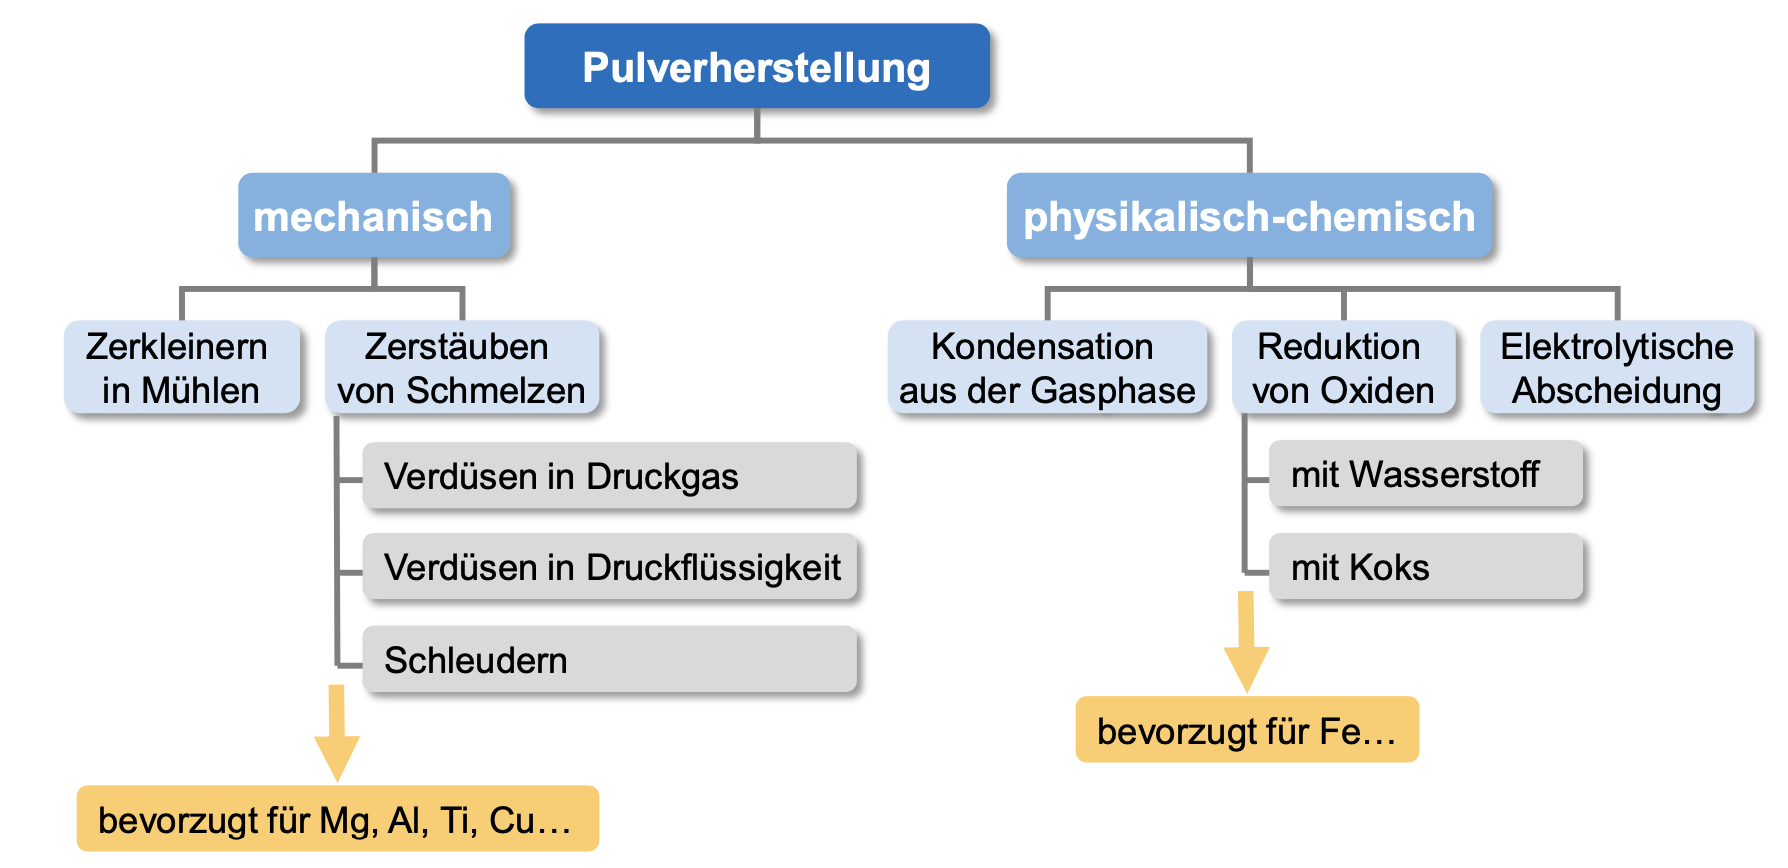
\includegraphics[width = 70mm]{src/images/Pulverherstellung.png}

\includegraphics[width = 70mm]{src/images/Verdüsen.png}
\begin{minipage}{0.5\linewidth}
    Verdüsen im Druckgas
    \begin{tiny}
        \begin{itemize}
            \item Kugelförmig
            \item 1 - 150 $\mu m$
        \end{itemize}
    \end{tiny}
\end{minipage}
\begin{minipage}{0.5\linewidth}
    Verdüsen in Druckflüssigkeit
    \begin{tiny}
        \begin{itemize}
            \item Unregelmäßig
            \item 50 - 500 $\mu m$
            \item Kostengünstig
        \end{itemize}
    \end{tiny}
\end{minipage}

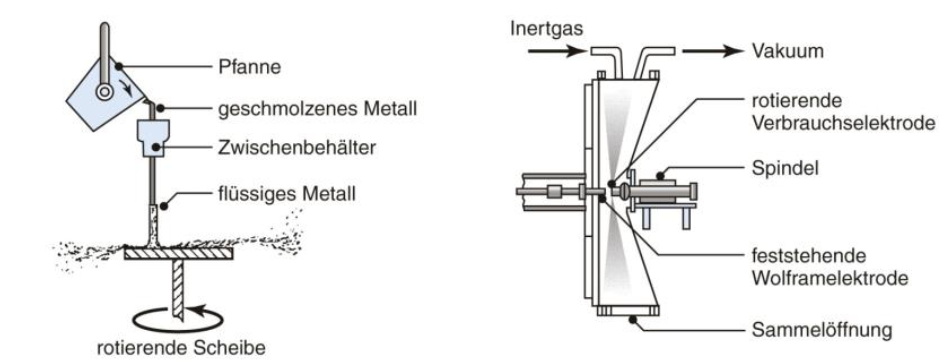
\includegraphics[width = 70mm]{src/images/Schleudern:Elektrolytisch.png}
\begin{minipage}{0.5\linewidth}
    Schleudern
    \begin{tiny}
        \begin{itemize}
            \item Kugelförmig
            \item 50 - 500 $\mu m$
            \item Kühlt Legierung schnell Abkühlrate
            \item Hohe Reinheit
        \end{itemize}
    \end{tiny}
\end{minipage}
\begin{minipage}{0.5\linewidth}
    Elektrolytische Abscheidung
    \begin{tiny}
        \begin{itemize}
            \item Kugelförmig
            \item 10 - 100 $\mu m$
            \item extrem fein
            \item Reines und gleichmässigs Pulver
        \end{itemize}
    \end{tiny}
\end{minipage}



